\chapter{Скобки Пуассона, генераторы и момент импульса}

\lectureoverview{Скобка Пуассона — это не просто компактный способ переписать уравнения Гамильтона. Это алгебраическая операция, порождающая преобразования. Скобка с гамильтонианом порождает эволюцию во времени; скобка с импульсом порождает трансляции; скобка с моментом импульса порождает вращения. На этом языке симметрия и закон сохранения становятся двумя прочтениями одного и того же равенства скобки нулю. Мы разовьём эту идею, начиная с гармонического осциллятора, а затем используем алгебру момента импульса, чтобы получить гироскопическую прецессию без введения углов Эйлера.}

\section{Функция вдоль гамильтоновой траектории}

Пусть
\[
  F=F(q_1,\ldots,q_n,p_1,\ldots,p_n)
\]
— достаточно гладкая функция на фазовом пространстве. Её можно рассматривать двояко. Во-первых, она ставит в соответствие число каждой точке фазового пространства. Во-вторых, после выбора гамильтоновой траектории она становится функцией времени, поскольку точка \((q(t),p(t))\) движется. Вдоль этой траектории
\begin{equation}
  \frac{dF}{dt}
  =
  \sum_i\left(
    \frac{\partial F}{\partial q_i}\dot q_i
    +\frac{\partial F}{\partial p_i}\dot p_i
  \right).
  \label{eq:l8-chain-rule}
\end{equation}
а уравнения Гамильтона,
\begin{equation}
  \dot q_i=\frac{\partial H}{\partial p_i},
  \qquad
  \dot p_i=-\frac{\partial H}{\partial q_i},
  \label{eq:l8-hamilton-equations}
\end{equation}
превращают это в
\begin{equation}
  \frac{dF}{dt}
  =
  \sum_i\left(
    \frac{\partial F}{\partial q_i}
    \frac{\partial H}{\partial p_i}
    -
    \frac{\partial F}{\partial p_i}
    \frac{\partial H}{\partial q_i}
  \right).
  \label{eq:l8-fdot-expanded}
\end{equation}
Комбинация в правой части встречается повсюду в классической механике, даже когда ни один из её аргументов не является гамильтонианом. Это мотивирует определение
\begin{equation}
  \boxed{
  \{F,G\}
  =
  \sum_i\left(
    \frac{\partial F}{\partial q_i}
    \frac{\partial G}{\partial p_i}
    -
    \frac{\partial F}{\partial p_i}
    \frac{\partial G}{\partial q_i}
  \right).}
  \label{eq:l8-poisson-definition}
\end{equation}
Поэтому уравнение~\eqref{eq:l8-fdot-expanded} принимает вид
\begin{equation}
  \boxed{\dot F=\{F,H\}.}
  \label{eq:l8-time-generator}
\end{equation}

\begin{classroomqa}
  \audiencequestion{Если второй аргумент заменить \(H\) на произвольную функцию \(G\), будет ли скобка по-прежнему производной \(F\) по времени?
  \lecturetimestamp{00:05:45--00:06:15}}
  \lecturerresponse{Нет. По мере обобщения обозначений аудитория улавливает важный момент. Уравнение~\eqref{eq:l8-poisson-definition}
  определяет \(\{F,G\}\) для любых двух функций на фазовом пространстве, но
  \(\dot F=\{F,G\}\) верно только тогда, когда \(G\) — гамильтониан. Произвольное
  \(G\) будет порождать другое бесконечно малое преобразование.}
\end{classroomqa}

Полезно записывать малое изменение во времени в виде
\begin{equation}
  \delta_t F=\epsilon\,\{F,H\}.
  \label{eq:l8-small-time-step}
\end{equation}
Эта форма предвосхищает то, что появится дальше. Эволюция во времени — лишь один представитель более широкого семейства преобразований, порождаемых скобками Пуассона.

\section{Алгебра скобок}

Теперь скобку можно использовать как самостоятельное исчисление. Её правила следуют из обычного дифференцирования:
\begin{align}
  \{A,B\}&=-\{B,A\}, \label{eq:l8-antisymmetry}\\
  \{A+B,C\}&=\{A,C\}+\{B,C\}, \label{eq:l8-additivity}\\
  \{\lambda A,B\}&=\lambda\{A,B\},
    \quad \lambda\ \text{constant}, \label{eq:l8-scalar-rule}\\
  \{AB,C\}&=A\{B,C\}+\{A,C\}B. \label{eq:l8-leibniz}
\end{align}
Эти четыре строки выражают соответственно антисимметрию, аддитивность, линейность при умножении на константу и правило Лейбница.
Классические функции на фазовом пространстве перемножаются коммутативно, поэтому расположение обычных множителей \(A\) и \(B\) в последней строке несущественно. Для операторов в квантовой механике это уже неверно. Антисимметрия также влечёт
\begin{equation}
  \{A,A\}=0.
  \label{eq:l8-self-bracket}
\end{equation}

Для канонических координат элементарные скобки имеют вид
\begin{equation}
  \boxed{
  \{q_i,q_j\}=0,\qquad
  \{p_i,p_j\}=0,\qquad
  \{q_i,p_j\}=\delta_{ij}.}
  \label{eq:l8-canonical-brackets}
\end{equation}
Любая функция только от \(q_i\) имеет нулевую скобку с любой другой функцией только от \(q_i\); аналогичное утверждение верно для функций только от \(p_i\). Чтобы скобка была ненулевой, каноническая координата должна встретиться со своим сопряжённым импульсом. Дельта Кронекера в ур.~\eqref{eq:l8-canonical-brackets} показывает, что встречаются только совпадающие индексы.

\subsection{Гармонический осциллятор как проверка}

Рассмотрим
\begin{equation}
  H=\frac{p^2}{2m}+\frac{kq^2}{2}.
  \label{eq:l8-oscillator-hamiltonian}
\end{equation}
Теперь мы намеренно используем только правила для скобок и
Eq.~\eqref{eq:l8-time-generator}. Сначала
\begin{align}
  \dot q
  &=\{q,H\}\\
  &=\frac{1}{2m}\{q,p^2\}\\
  &=\frac{1}{2m}\left(p\{q,p\}+\{q,p\}p\right)\\
  &=\frac{p}{m}.
  \label{eq:l8-qdot-oscillator}
\end{align}
Член потенциальной энергии исчезает, поскольку \(\{q,q^2\}=0\). Аналогично,
\begin{align}
  \dot p
  &=\{p,H\}\\
  &=\frac{k}{2}\{p,q^2\}\\
  &=\frac{k}{2}\left(q\{p,q\}+\{p,q\}q\right)\\
  &=-kq.
  \label{eq:l8-pdot-oscillator}
\end{align}
Знак минус — это как раз антисимметрия
\(\{p,q\}=-\{q,p\}=-1\). Объединяя два уравнения первого порядка, получаем
\begin{equation}
  m\ddot q=-kq.
  \label{eq:l8-hooke-equation}
\end{equation}

\begin{figure}[htbp]
  \centering
  
\includegraphics[width=0.82\textwidth]{lecture_08_figure_01.png}
  \caption{Гамильтониан осциллятора и два вычисления скобок, дающие
  \(\dot q=p/m\) и \(\dot p=-kq\).}
  \lectureframe{00:23:20}
\end{figure}

Во время вычисления аудитория ищет глагол, означающий
\emph{take a Poisson bracket}, и временно останавливается на
\emph{Poissonate}. Эта шутка отмечает реальное изменение точки зрения: как только алгебра известна, с ней можно работать напрямую, вместо того чтобы заново выводить каждый результат из определения.

\begin{classroomqa}
  \audiencequestion{Является ли эта математическая структура группой или алгеброй?
  Есть ли у неё обратные элементы? \lecturetimestamp{00:23:48--00:24:16}}
  \lecturerresponse{Это не группа: операция скобки не даёт
  требуемых нейтрального элемента и обратных элементов. Функции на
  фазовом пространстве образуют алгебру Пуассона: у них есть обычные
  коммутативные умножение и сложение, а также антисимметричная скобка,
  подчиняющаяся правилу Лейбница. Дополнительное тождество —
  тождество Якоби — завершает обычное абстрактное определение,
  хотя в этой лекции оно не разбирается.}
\end{classroomqa}

\begin{classroomqa}
  \audiencequestion{Какова связь между скобками Пуассона и
  квантовыми коммутаторами? \lecturetimestamp{00:24:18--00:25:00}}
  \lecturerresponse{Лекция даёт лишь предварительное представление. При переходе к
  квантовой механике классическая скобка схематически заменяется на
  \[
    \{A,B\}_{\mathrm{PB}}
    \longleftrightarrow
    \frac{1}{i\hbar}[\widehat A,\widehat B].
  \]
  Это соответствие требует оговорок относительно упорядочения операторов и
  квантования; здесь оно не используется как теорема.}
\end{classroomqa}

Для осциллятора скобка лишь заново воспроизвела уравнения Гамильтона.
Её подлинная экономичность проявляется, когда генератором служит сохраняющаяся величина, отличная от
\(H\).

\section{Восстановление момента импульса из вращательной симметрии}

Напомним бесконечно малую форму нётеровской конструкции, использованную ранее в курсе. Если непрерывная симметрия изменяет координаты по закону
\begin{equation}
  \delta q_i=\epsilon F_i(q),
  \label{eq:l8-noether-variation}
\end{equation}
то в рассматриваемой здесь постановке соответствующая сохраняющаяся величина равна
\begin{equation}
  G=\sum_i p_iF_i(q).
  \label{eq:l8-noether-charge}
\end{equation}
Общий множитель \(\epsilon\) можно опустить: умножение сохраняющейся величины на фиксированное число не меняет закона сохранения.

Возьмём одну частицу и выполним бесконечно малый поворот вокруг оси \(z\). При ориентации, принятой в лекции,
\begin{equation}
  \delta x=-\epsilon y,\qquad
  \delta y=\epsilon x,\qquad
  \delta z=0.
  \label{eq:l8-z-rotation}
\end{equation}
Уравнение~\eqref{eq:l8-noether-charge} даёт
\begin{equation}
  L_z=-p_xy+p_yx=xp_y-yp_x.
  \label{eq:l8-lz}
\end{equation}
Циклически переставляя \(x\), \(y\) и \(z\),
\begin{equation}
  \boxed{\begin{aligned}
    L_x&=yp_z-zp_y,\\
    L_y&=zp_x-xp_z,\\
    L_z&=xp_y-yp_x.
  \end{aligned}}
  \label{eq:l8-angular-components}
\end{equation}
Это компоненты
\begin{equation}
  \boldsymbol L=\boldsymbol r\times\boldsymbol p.
  \label{eq:l8-cross-product}
\end{equation}

\begin{figure}[htbp]
  \centering
  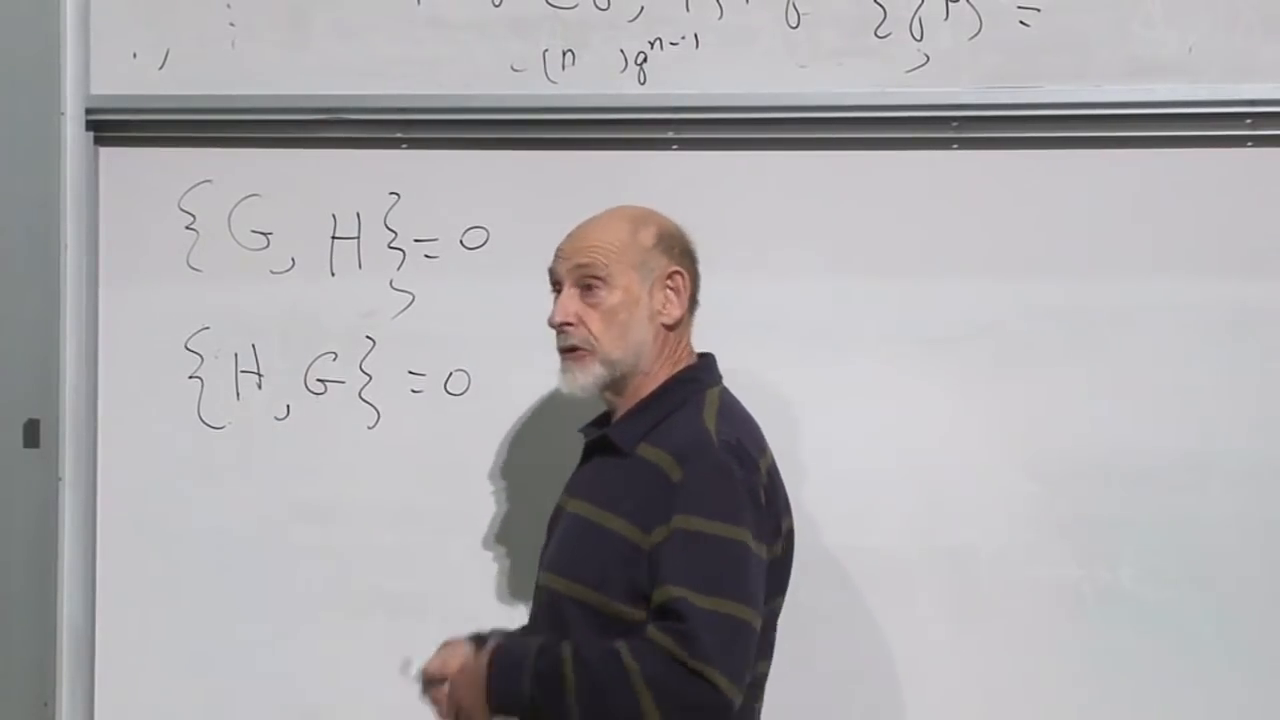
\includegraphics[width=0.82\textwidth]{lecture_08_figure_02.png}
  \caption{Три декартовы компоненты момента импульса и их компактная форма через векторное произведение.}
  \lectureframe{00:34:00}
\end{figure}

Вращение вокруг оси, заданной произвольным единичным вектором \(\boldsymbol n\), порождается
\begin{equation}
  L_{\boldsymbol n}=\boldsymbol n\cdot\boldsymbol L.
  \label{eq:l8-arbitrary-axis}
\end{equation}
Для изолированной вращательно-инвариантной системы сохраняются все три компоненты. Если симметрией остаются только вращения вокруг одной оси, то гарантированно сохраняется лишь компонента вдоль этой оси.

\section{Момент импульса порождает вращения}

Вместо того чтобы сразу решать задачу о вращательной динамике, исследуем, как \(L_z\) действует через скобку Пуассона. Используя
Eq.~\eqref{eq:l8-lz},
\begin{align}
  \{x,L_z\}
  &=\{x,xp_y-yp_x\}
   =-y\{x,p_x\}
   =-y,\\
  \{y,L_z\}
  &=\{y,xp_y-yp_x\}
   =x\{y,p_y\}
   =x,\\
  \{z,L_z\}&=0.
  \label{eq:l8-position-rotation-brackets}
\end{align}
Это в точности коэффициенты из
Eq.~\eqref{eq:l8-z-rotation}.

\begin{figure}[htbp]
  \centering
  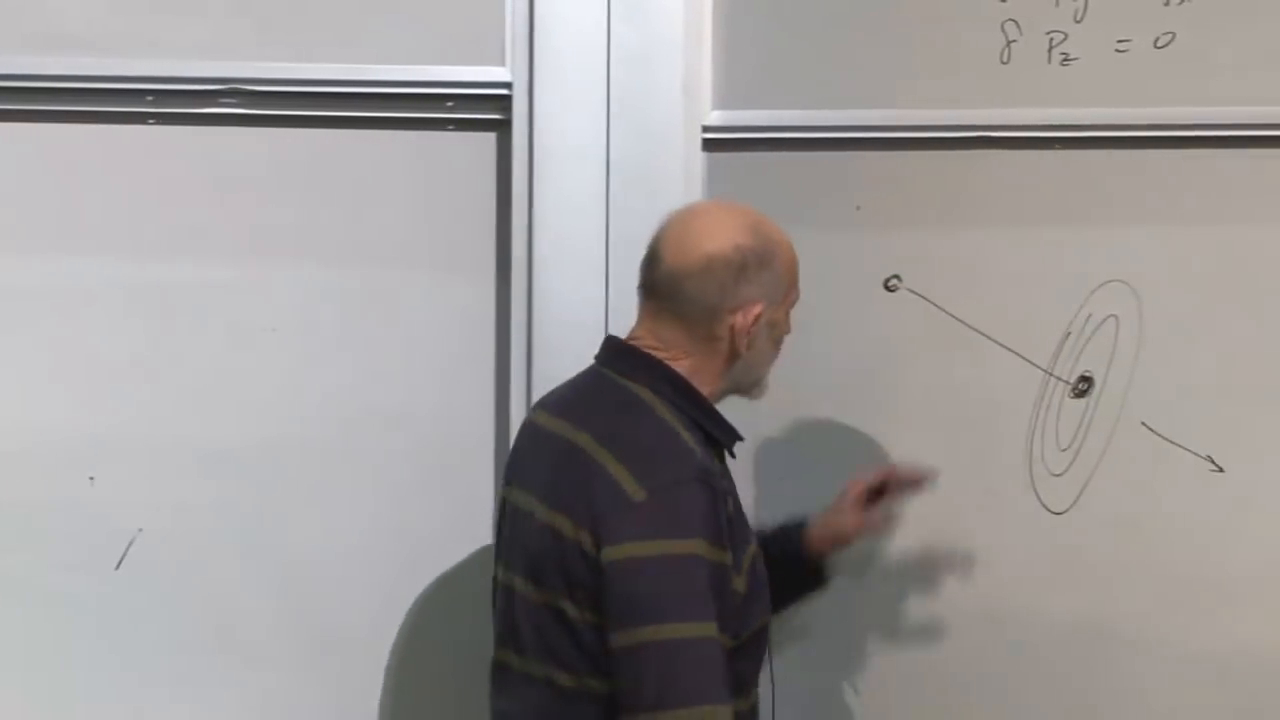
\includegraphics[width=0.82\textwidth]{lecture_08_figure_03.png}
  \caption{Скобки координат с \(L_z\): скобка воспроизводит бесконечно малый поворот \((x,y,z)\).}
  \lectureframe{00:38:41}
\end{figure}

Импульс тоже является вектором, и тот же расчёт даёт
\begin{equation}
  \begin{aligned}
    \{p_x,L_z\}&=-p_y,\\
    \{p_y,L_z\}&=p_x,\\
    \{p_z,L_z\}&=0.
  \end{aligned}
  \label{eq:l8-momentum-rotation-brackets}
\end{equation}

\begin{figure}[htbp]
  \centering
  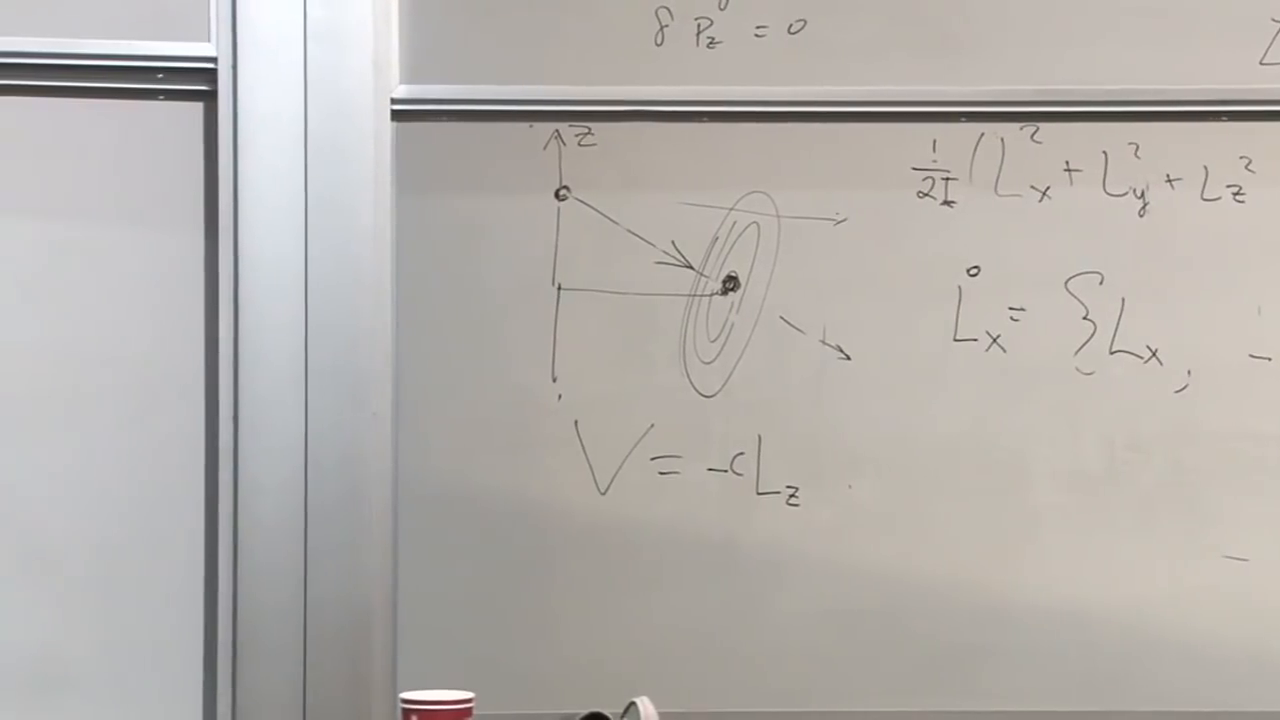
\includegraphics[width=0.82\textwidth]{lecture_08_figure_04.png}
  \caption{Положение и импульс преобразуются по одному и тому же векторному закону при вращении, порождаемом \(L_z\).}
  \lectureframe{00:42:08}
\end{figure}

Итак, общее утверждение гамильтоновой механики таково:
\begin{equation}
  \boxed{\delta_G A=\epsilon\{A,G\}.}
  \label{eq:l8-generator-rule}
\end{equation}
Каждая функция фазового пространства \(G\) задаёт такое бесконечно малое каноническое преобразование. Если \(G=L_z\), это вращение. Если \(G=H\), это малый шаг по времени.

\begin{classroomqa}
  \audiencequestion{В лекции иногда говорится о вращении системы и
  иногда — о вращении координат. Какое соглашение используется в уравнениях со скобками?
  \lecturetimestamp{00:28:22--00:29:35}}
  \lecturerresponse{Уравнение~\eqref{eq:l8-z-rotation} фиксирует соглашение:
  речь идёт об активном бесконечно малом повороте
  \((x,y)\mapsto(x-\epsilon y,y+\epsilon x)\). Пассивный поворот осей
  даёт противоположный знак. Как только соглашение зафиксировано, формулы со скобками становятся однозначными.}
\end{classroomqa}

\section{Импульс порождает трансляции}

Трансляция по одной координате имеет вид
\begin{equation}
  \delta q=\epsilon.
  \label{eq:l8-q-translation}
\end{equation}
Здесь \(F(q)=1\) в Eq.~\eqref{eq:l8-noether-variation}, поэтому соответствующая
сохраняющаяся величина — \(p\). Утверждение о генераторе предсказывает
\begin{equation}
  \{f(q),p\}=\frac{df}{dq}.
  \label{eq:l8-translation-derivative}
\end{equation}
В лекции это сначала доказывается для степеней методом индукции. База индукции —
\(\{q,p\}=1\). Предположим,
\begin{equation}
  \{q^{n-1},p\}=(n-1)q^{n-2}.
  \label{eq:l8-induction-hypothesis}
\end{equation}
Тогда правило произведения даёт
\begin{align}
  \{q^n,p\}
  &=\{q\,q^{n-1},p\}\\
  &=q\{q^{n-1},p\}+\{q,p\}q^{n-1}\\
  &=(n-1)q^{n-1}+q^{n-1}\\
  &=nq^{n-1}.
  \label{eq:l8-power-translation}
\end{align}
По линейности результат распространяется на многочлены и на сходящиеся представления степенными рядами.
Ещё прямее, определение скобки даёт
Eq.~\eqref{eq:l8-translation-derivative} для любой дифференцируемой \(f(q)\):
\begin{equation}
  \{f(q),p\}
  =
  \frac{\partial f}{\partial q}
  \frac{\partial p}{\partial p}
  =f'(q).
\end{equation}

\begin{figure}[htbp]
  \centering
  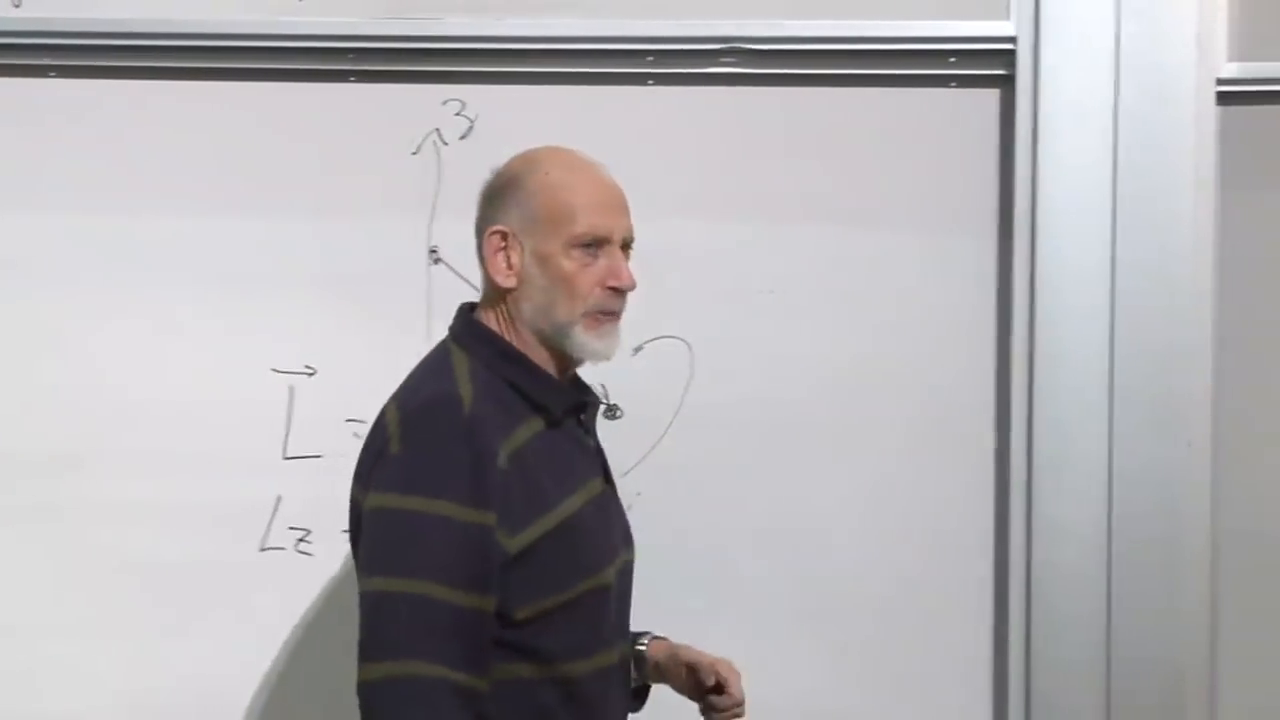
\includegraphics[width=0.82\textwidth]{lecture_08_figure_05.png}
  \caption{Результат для трансляции после индукционного доказательства:
  \(\{F(q),p\}=dF/dq\).}
  \lectureframe{00:53:18}
\end{figure}

Теперь мы увидели три варианта одной и той же идеи:
\begin{center}
  \begin{tabular}{@{}>{\raggedright\arraybackslash}p{0.37\textwidth}
                      >{\raggedright\arraybackslash}p{0.55\textwidth}@{}}
    \toprule
    Генератор и преобразование&Бесконечно малое действие\\
    \midrule
    \(H\), сдвиг по времени& \(\delta_tA=\epsilon\{A,H\}\)\\
    \(p_i\), пространственный сдвиг& \(\delta A=\epsilon\{A,p_i\}\)\\
    \(L_i\), вращение& \(\delta A=\epsilon\{A,L_i\}\)\\
    \bottomrule
  \end{tabular}
\end{center}
Сохраняющаяся величина, связанная с непрерывной симметрией, также является генератором этой симметрии.

\section{Одна скобка, два прочтения}

Пусть \(G(q,p)\) — предполагаемый генератор. Если он сохраняется и не имеет явной зависимости от времени, то
\begin{equation}
  \dot G=\{G,H\}=0.
  \label{eq:l8-g-conserved}
\end{equation}
По антисимметрии,
\begin{equation}
  \{H,G\}=0.
  \label{eq:l8-h-invariant}
\end{equation}
Эти уравнения математически эквивалентны, но их физический смысл различен:
\begin{itemize}
  \item \(\{G,H\}=0\) утверждает, что \(G\) не меняется при временной эволюции, порождённой \(H\).
  \item \(\{H,G\}=0\) утверждает, что \(H\) не меняется при преобразовании, порождённом \(G\).
\end{itemize}
Первое — закон сохранения; второе — симметрия гамильтониана. Связь Нётер здесь сжата до одного нуля.

\begin{figure}[htbp]
  \centering
  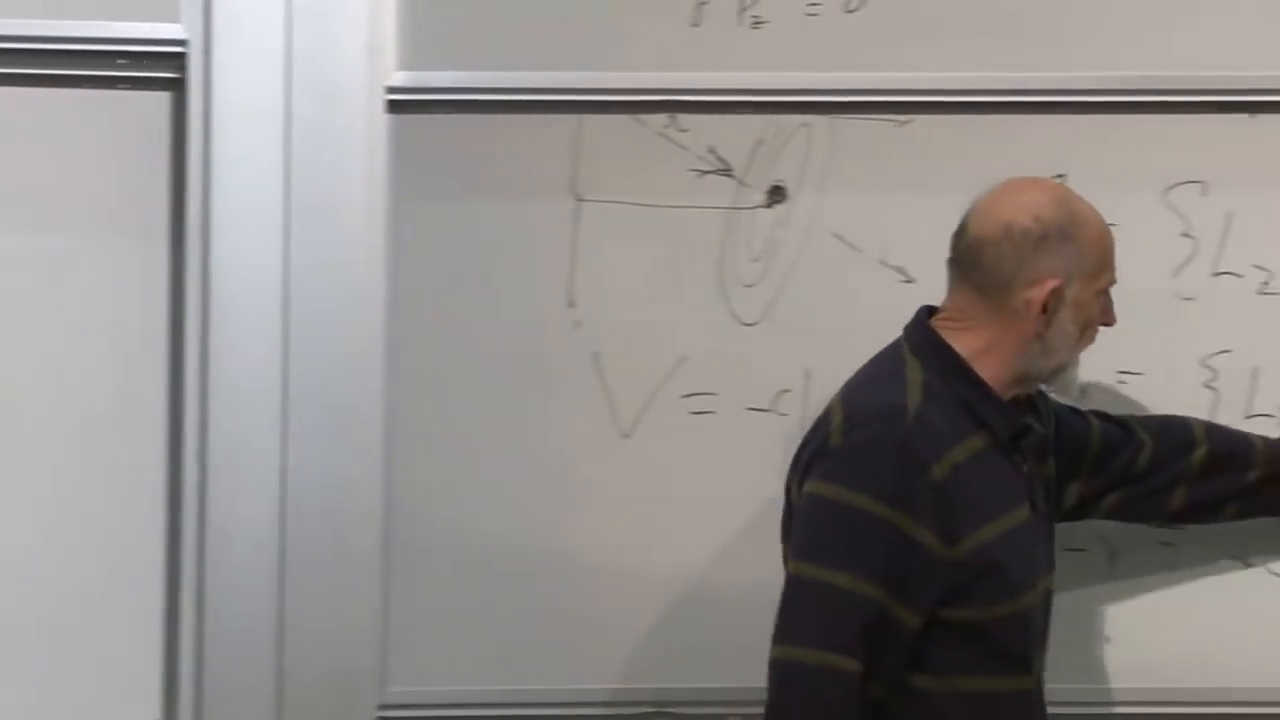
\includegraphics[width=0.82\textwidth]{lecture_08_figure_06.png}
  \caption{Два порядка одной и той же обращающейся в нуль скобки: сохранение \(G\) и инвариантность \(H\) относительно преобразования, порождённого \(G\).}
  \lectureframe{01:03:05}
\end{figure}

\begin{classroomqa}
  \audiencequestion{Если известна сохраняющаяся величина, всегда ли можно восстановить соответствующую симметрию? \lecturetimestamp{01:01:42--01:02:15}}
  \lecturerresponse{В рамках этой гамильтоновой постановки — да: возьмите скобку каждой переменной фазового пространства с \(G\). Совокупность соотношений \(\delta_GA=\epsilon\{A,G\}\) показывает, как преобразуются переменные. Например, скобки с \(L_z\) выявляют вращение, даже если такая интерпретация заранее не была известна. В более сложных постановках возможны глобальные и граничные тонкости, но здесь используется именно локальное инфинитезимальное утверждение.}
\end{classroomqa}

\begin{classroomqa}
  \audiencequestion{Говорят ли эти уравнения со скобками, какое физическое движение отвечает за закон сохранения?
  \lecturetimestamp{00:56:01--00:58:13}}
  \lecturerresponse{Нет. Они задают преобразование симметрии, а не фактическую траекторию. Сохранение \(L_z\) указывает на вращательную симметрию; оно не означает, что частица движется по окружности. Реальную временную эволюцию порождает \(H\). Скобка с другим генератором описывает другое направление преобразования в фазовом пространстве.}
\end{classroomqa}

\begin{classroomqa}
  \audiencequestion{Существует ли общее утверждение о преобразовании, которое не предполагает сохранения заранее? \lecturetimestamp{01:02:40--01:04:45}}
  \lecturerresponse{Да. Уравнение~\eqref{eq:l8-generator-rule} определяет инфинитезимальное преобразование для любой функции \(G\), независимо от того, сохраняется она или нет. Оно становится симметрией только тогда, когда гамильтониан инвариантен: \(\{H,G\}=0\). То же условие, прочитанное в обратном порядке, тогда утверждает, что \(G\) сохраняется.}
\end{classroomqa}

\section{Алгебра углового момента}

Следующее вычисление избавляет нас от необходимости протаскивать координаты частицы через каждую задачу о вращении. Начнём с
\[
  L_x=yp_z-zp_y,\qquad
  L_z=xp_y-yp_x.
\]
В \(\{L_x,L_z\}\) большинство перекрёстных членов обращается в нуль, потому что их индексы не образуют канонических пар. Оставшиеся свёртки дают
\begin{align}
  \{L_x,L_z\}
  &=\{yp_z-zp_y,xp_y-yp_x\}\\
  &=xp_z-zp_x\\
  &=-L_y.
  \label{eq:l8-lx-lz}
\end{align}
При обращении порядка минус исчезает. Циклическая перестановка координат даёт
\begin{equation}
  \boxed{\begin{aligned}
    \{L_x,L_y\}&=L_z,\\
    \{L_y,L_z\}&=L_x,\\
    \{L_z,L_x\}&=L_y.
  \end{aligned}}
  \label{eq:l8-angular-algebra}
\end{equation}
В индексной записи,
\begin{equation}
  \{L_i,L_j\}=\varepsilon_{ijk}L_k.
  \label{eq:l8-angular-algebra-index}
\end{equation}

\begin{figure}[htbp]
  \centering
  \includegraphics[width=0.82\textwidth]{lecture_08_figure_07.png}
  \caption{Циклическая алгебра скобок Пуассона трёх компонент углового момента.}
  \lectureframe{01:10:52}
\end{figure}

Этот результат можно было и предвидеть. Поскольку \(\boldsymbol L\) — вектор, скобка её \(x\)-компоненты с \(L_z\) должна давать инфинитезимальное изменение этой компоненты при вращении вокруг \(z\), а именно \(-L_y\). Явное вычисление подтверждает этот геометрический аргумент. Эти уравнения также являются классическими предшественниками квантовых коммутационных соотношений для углового момента.

\section{Быстрый гироскоп}

В качестве применения рассмотрим гироскоп: быстро вращающийся маховик, центр которого находится на фиксированном расстоянии \(R\) от точки опоры. Пусть \(\boldsymbol r\) направлен от опоры к центру колеса. Маховик вращается вокруг своей оси настолько быстро, что его основной угловой момент остаётся направленным вдоль этого направления. В приближении, используемом в лекции,
\begin{equation}
  \boldsymbol L=\ell\,\boldsymbol r,
  \qquad
  L_z=\ell z,
  \label{eq:l8-L-parallel-r}
\end{equation}
где \(\ell=L/R\) считается постоянной. Меньшими угловыми моментами, связанными с нутацией или движением оси, поначалу пренебрегают.

\begin{figure}[htbp]
  \centering
  \begin{tikzpicture}[scale=0.95,>=Latex]
    \coordinate (P) at (0,3.2);
    \coordinate (C) at (3.7,1.55);
    \draw[->] (0,-0.2) -- (0,4.35) node[above] {\(z\)};
    \fill (P) circle (1.7pt) node[left] {pivot};
    \draw[very thick,->] (P) -- (C)
      node[midway,above right] {\(\boldsymbol r\parallel\boldsymbol L\)};
    \fill (C) circle (1.7pt);
    \draw[dashed] (P) -- (0,1.55);
    \draw[dashed] (0,1.55) -- (C);
    \node[left] at (0,1.55) {\(z\)};
    \begin{scope}[shift={(C)},rotate=-24]
      \draw[very thick] (0,0) ellipse (0.65 and 1.35);
      \draw[thick] (0,0) ellipse (0.42 and 0.9);
    \end{scope}
    \draw[->,thick] (2.15,2.85)
      arc[start angle=140,end angle=35,radius=1.65];
  \end{tikzpicture}
  \caption{Приближение быстрого гироскопа. Расстояние от опоры до центра фиксировано, а доминирующий момент собственного вращения остаётся сонаправленным с осью и \(\boldsymbol r\).}
\end{figure}

\begin{figure}[htbp]
  \centering
  \includegraphics[width=0.82\textwidth]{lecture_08_figure_08.png}
  \caption{Эскиз маховика на доске вместе с \(H_{\rm rot}=L^2/(2I)\) и сокращением членов, доказывающим сохранение \(\boldsymbol L\) при отсутствии момента сил.}
  \lectureframe{01:18:54}
\end{figure}

\subsection{Без гравитации: почему каждая компонента остаётся постоянной}

Для упрощённого осесимметричного ротора
\begin{equation}
  H_{\mathrm{rot}}
  =\frac{1}{2I}
  \left(L_x^2+L_y^2+L_z^2\right)
  =\frac{L^2}{2I}.
  \label{eq:l8-rotational-hamiltonian}
\end{equation}
Коэффициент равен \(1/(2I)\), а не \(I/2\); на доске эта ошибка появляется и исправляется. Используя уравнение~\eqref{eq:l8-angular-algebra},
\begin{align}
  \dot L_x
  &=\{L_x,H_{\mathrm{rot}}\}\\
  &=\frac{1}{2I}\left(
    2L_y\{L_x,L_y\}
    +2L_z\{L_x,L_z\}
  \right)\\
  &=\frac{1}{I}\left(L_yL_z-L_zL_y\right)=0.
  \label{eq:l8-free-lx}
\end{align}
При циклической перестановке,
\begin{equation}
  \dot L_x=\dot L_y=\dot L_z=0.
  \label{eq:l8-free-angular-momentum}
\end{equation}
Скаляр \(L^2\) имеет нулевую скобку с каждой компонентой \(L_i\); на языке этой алгебры это элемент Казимира. Следовательно, гироскоп без момента сил сохраняет и модуль, и направление своего углового момента.

\begin{classroomqa}
  \audiencequestion{Является ли момент инерции здесь просто числом?
  \lecturetimestamp{01:14:23--01:15:05}}
  \lecturerresponse{Для этой редуцированной модели — да. Он кодирует распределение массы колеса относительно его оси вращения. Для общего твёрдого тела имеется тензор моментов инерции и вращательный гамильтониан \(\sum_i L_i^2/(2I_i)\) в главных осях. В лекции выбирается более простой быстрый симметричный ротор, потому что цель состоит в том, чтобы показать метод скобок Пуассона, а не развивать полную динамику твёрдого тела.}
\end{classroomqa}

\subsection{Гравитация и знак потенциала}

Выберем вертикальную координату \(z\) положительной вверх и поместим точку опоры в начало координат. Потенциальная энергия тяжести центра колеса равна
\begin{equation}
  V=Mgz.
  \label{eq:l8-mgz}
\end{equation}
Поскольку \(L_z=\ell z\),
\begin{equation}
  V=cL_z,
  \qquad
  c=\frac{Mg}{\ell}=\frac{MgR}{L}.
  \label{eq:l8-potential-lz}
\end{equation}
Здесь \(c>0\), если \(\boldsymbol L\) выбрано параллельным \(\boldsymbol r\). Если маховик вращается в противоположную сторону, знаковая связь между \(\boldsymbol L\) и \(\boldsymbol r\) меняется на противоположную, и то же происходит с соответствующей знаковой частотой прецессии.

\begin{figure}[htbp]
  \centering
  \includegraphics[width=0.82\textwidth]{lecture_08_figure_09.png}
  \caption{Геометрия при фиксированной длине, лежащая в основе \(\boldsymbol L=\ell\boldsymbol r\) и \(L_z=\ell z\).}
  \lectureframe{01:25:38}
\end{figure}

\begin{figure}[htbp]
  \centering
  \includegraphics[width=0.82\textwidth]{lecture_08_figure_10.png}
  \caption{На промежуточном этапе на доске записано \(V=-cL_z\). Позднее знак исправляется после того, как \(z\) фиксируется направленной вверх: при \(\boldsymbol L=\ell\boldsymbol r\) и \(\ell>0\) согласованный результат таков: \(V=+cL_z\).}
  \lectureframe{01:22:43}
\end{figure}

\begin{classroomqa}
  \audiencequestion{Почему высоту можно заменить компонентой углового момента? Наклонная линия — это ось или радиус-вектор?
  \lecturetimestamp{01:22:20--01:25:43}}
  \lecturerresponse{Наклонную линию лучше всего обозначить как \(\boldsymbol r\), вектор от закреплённой опоры к центру колеса. Реальная ось может лежать вдоль него, но соотношение, используемое в вычислении, — это приближение быстрого вращения \(\boldsymbol L=\ell\boldsymbol r\). Поэтому их \(z\)-компоненты пропорциональны. В живом обсуждении обозначения несколько раз меняются, прежде чем это различие окончательно фиксируется.}
\end{classroomqa}

\begin{classroomqa}
  \audiencequestion{Какие предположения делают \(\ell\) постоянной, и что перестаёт работать, если центр колеса может скользить радиально?
  \lecturetimestamp{01:25:43--01:26:38,\allowbreak\ 01:34:22--01:35:00}}
  \lecturerresponse{Предполагается, что доминирующий угловой момент собственного вращения намного больше углового момента, связанного с медленным движением, а расстояние от опоры до центра фиксировано. Тогда модуль собственного вращения мало меняется, и \(\boldsymbol L\) вращается вместе с \(\boldsymbol r\). Если бы центр мог скользить радиально, \(z\) уже не было бы пропорционально \(L_z\) с одним постоянным коэффициентом, так что редуцированный гамильтониан \(V=cL_z\) не описывал бы движение.}
\end{classroomqa}

\begin{classroomqa}
  \audiencequestion{Почему на доске сначала стоит минус, а позже плюс? Имеет ли направление вращения значение?
  \lecturetimestamp{01:27:13--01:28:15,\allowbreak\ 01:33:09--01:33:21}}
  \lecturerresponse{Начальный знак — это ошибка на доске по ходу лекции, смешанная с ещё не устоявшейся договорённостью о направлении оси. Как только \(z\) определяется направленной вверх, \(V=Mgz\) растёт с высотой. Если \(\boldsymbol L=\ell\boldsymbol r\) при \(\ell>0\), получаем \(V=+cL_z\). При обращении направления вращения меняются на противоположные знаковая пропорциональность и направление прецессии, но это не возвращает возможности произвольно выбирать знак.}
\end{classroomqa}

\subsection{Прецессия из трёх коротких уравнений}

Полный редуцированный гамильтониан имеет вид
\begin{equation}
  H=
  \frac{1}{2I}\left(L_x^2+L_y^2+L_z^2\right)+cL_z.
  \label{eq:l8-full-gyro-hamiltonian}
\end{equation}
Мы уже показали, что \(L^2\) имеет нулевую скобку с каждым \(L_i\). Вклад даёт только линейный член:
\begin{align}
  \dot L_z&=\{L_z,H\}=0,\\
  \dot L_x&=\{L_x,H\}=c\{L_x,L_z\}=-cL_y,\\
  \dot L_y&=\{L_y,H\}=c\{L_y,L_z\}=cL_x.
  \label{eq:l8-precession-equations}
\end{align}

\begin{figure}[htbp]
  \centering
  \includegraphics[width=0.82\textwidth]{lecture_08_figure_11.png}
  \caption{Итоговые уравнения для компонент: \(L_z\) постоянно, тогда как \(L_x\) и \(L_y\) переходят друг в друга при вращении.}
  \lectureframe{01:30:35}
\end{figure}

Вертикальная компонента и горизонтальный модуль постоянны:
\begin{equation}
  \frac{d}{dt}(L_x^2+L_y^2)
  =2L_x(-cL_y)+2L_y(cL_x)=0.
\end{equation}
Объединив горизонтальные компоненты,
\begin{equation}
  L_+=L_x+iL_y,
  \qquad
  \dot L_+=icL_+,
\end{equation}
поэтому
\begin{equation}
  L_+(t)=L_+(0)e^{ict}.
  \label{eq:l8-precession-solution}
\end{equation}
Следовательно, вектор углового момента прецессирует вокруг вертикальной оси с угловой скоростью \(|c|=MgR/L\). В этом идеализированном стационарном движении его наклон остаётся постоянным.

\begin{classroomqa}
  \audiencequestion{Был ли опущен член вращательной энергии, когда записывались уравнения прецессии?
  \lecturetimestamp{01:35:01--01:35:49}}
  \lecturerresponse{Нет. Он входит в полный гамильтониан, как в формуле~\eqref{eq:l8-full-gyro-hamiltonian}. Он просто даёт нулевой вклад в \(\dot L_i\), поскольку \(\{L_i,L^2\}=0\); это сокращение уже было доказано в расчёте без момента сил. Вопрос студента делает этот неявный шаг явным.}
\end{classroomqa}

\begin{classroomqa}
  \audiencequestion{Является ли равномерная прецессия равновесием? Что происходит после небольшого толчка? \lecturetimestamp{01:32:38--01:33:08}}
  \lecturerresponse{Её лучше называть установившимся или стационарным движением, а не статическим равновесием. Небольшой толчок, вообще говоря, добавляет нутацию, то есть колебание угла наклона. Для очень быстро вращающегося колеса это колебание мало, поэтому в сокращённом рассмотрении сохраняют только почти равномерную прецессию.}
\end{classroomqa}

\begin{classroomqa}
  \audiencequestion{Требует ли прецессия опоры или реальной оси?
  \lecturetimestamp{01:31:49--01:32:38,\allowbreak\ 01:33:49--01:35:00}}
  \lecturerresponse{В этой механической модели предполагается фиксированное расстояние от шарнира до центра, так что опору обеспечивает некоторая связь. Более глубокий алгебраический результат шире: всякий раз, когда гамильтониан содержит член, линейный по одной из компонент углового момента, та же алгебра скобок порождает прецессию. Микроскопический источник углового момента не обязан быть буквально колесом на оси.}
\end{classroomqa}

\begin{classroomqa}
  \audiencequestion{Это та же прецессия, что и у электронного или ядерного спина в магнитном поле, или у орбиты планеты?
  \lecturetimestamp{01:35:50--01:37:00}}
  \lecturerresponse{Магнитный момент, взаимодействующий с магнитным полем, имеет гамильтониан, линейный по компоненте спина, и потому подчиняется той же алгебре углового момента. Прецессия ядерного спина лежит в основе ядерного магнитного резонанса. Прецессия перигелия планетной орбиты — другое явление, которое лишь обозначается тем же словом \emph{прецессия}; это не тот же расчёт.}
\end{classroomqa}

\begin{classroomqa}
  \audiencequestion{Является ли гироскоп с боковым креплением по существу тем же самым объектом, что и волчок? \lecturetimestamp{01:37:02--01:37:23}}
  \lecturerresponse{Да. Различие в основном в геометрической терминологии: когда ось вращения выступает в сторону от опоры, обычно говорят о гироскопе; когда она почти вертикальна, говорят о волчке. Структура углового момента и момента сил одна и та же.}
\end{classroomqa}

\section{Что дал этот расчёт}

Углы Эйлера не вводились, и координаты каждой части колеса не отслеживались. Как только стало известно
\[
  \{L_i,L_j\}=\varepsilon_{ijk}L_k
\]
, уравнения для интересующих переменных следовали непосредственно.
В этом и состояла задуманная демонстрация силы метода. Осциллятор показал, что скобки Пуассона могут воспроизводить знакомую динамику. Угловой момент показал, что они способны на гораздо большее:
\begin{itemize}
  \item сохраняющаяся величина порождает соответствующую ей бесконечно малую симметрию;
  \item сохранение \(G\) и инвариантность \(H\) — два прочтения \(\{G,H\}=0\);
  \item алгебра наблюдаемых может замыкаться на себя, что позволяет решать динамику, не возвращаясь к микроскопическим координатам;
  \item гамильтониан, линейный по одной из компонент углового момента, порождает прецессию вокруг этой оси.
\end{itemize}
Лекция останавливается, не доходя до полных уравнений Эйлера для общего твёрдого тела. Её более узкий вывод уже завершён: правильно выбранные генераторы и их алгебра Пуассона с поразительной экономией выявляют и симметрию, и движение.